\let\negmedspace\undefined
\let\negthickspace\undefined
\documentclass[journal,12pt,onecolumn]{IEEEtran}
\usepackage{cite}
\usepackage{amsmath,amssymb,amsfonts,amsthm}
\usepackage{algorithmic}
\usepackage{graphicx}
\graphicspath{{Figs/}}
\usepackage{textcomp}
\usepackage{xcolor}
\usepackage{txfonts}
\usepackage{listings}
\usepackage{enumitem}
\usepackage{mathtools}
\usepackage{gensymb}
\usepackage{comment}
\usepackage{caption}
\usepackage[breaklinks=true]{hyperref}
\usepackage{tkz-euclide} 
\usepackage{listings}
\usepackage{gvv}                                        
%\def\inputGnumericTable{}                                 
\usepackage[latin1]{inputenc}     
\usepackage{xparse}
\usepackage{color}                                            
\usepackage{array}                                            
\usepackage{longtable}                                       
\usepackage{calc}                                             
\usepackage{multirow}
\usepackage{multicol}
\usepackage{hhline}                                           
\usepackage{ifthen}                                           
\usepackage{lscape}
\usepackage{tabularx}
\usepackage{array}
\usepackage{float}
%\newtheorem{theorem}{Theorem}[section]
%\newtheorem{theorem}{Theorem}[section]
%\newtheorem{problem}{Problem}
%\newtheorem{proposition}{Proposition}[section]
%\newtheorem{lemma}{Lemma}[section]
%\newtheorem{corollary}[theorem]{Corollary}
%\newtheorem{example}{Example}[section]
%\newtheorem{definition}[problem]{Definition}

\begin{document}

\title{2.9.18}
\author{AI25BTECH11002 - Ayush Sunil Labhade}
{\let\newpage\relax\maketitle}
%\renewcommand{\thefigure}{\theenumi}
%\renewcommand{\thetable}{\theenumi}
		\textbf{Question}:\newline

		Find the volume of a cuboid whose edges are given by  $-3\hat{\imath}+7\hat{\jmath}+5\hat{k}$,  $-5\hat{\imath}+7\hat{\jmath}-3\hat{k}$ and  $7\hat{\imath}-5\hat{\jmath}-3\hat{k}$.
		\newline
		\textbf{Solution:}
		Given:
		\begin{table}[H]
			\centering
			\begin{tabular}{|c|c|}
\hline
Point & Vector \\
\hline
$\vec{a}$ & $\myvec{3 \\ 7 \\ 5}$ \\
\hline
$\vec{b}$ & $\myvec{-5 \\ 7 \\ -3}$ \\
\hline
$\vec{c}$ & $\myvec{7 \\ -5 \\ -3}$ \\
\hline
\end{tabular}

			\label{}
			\caption{Given data}
		\end{table}
		To find volume we need to compute \sbrak{a \ b \ c}
		We will compute by finding the determinant of \sbrak{a \ b \ c}:
		\begin{align}
			\vec{D}=\myvec{a & b & c}
		\end{align}
		\begin{align}
			\vec{D} =
		\myvec{
3 & -5 & -7 \\
7 & 7 & -5 \\
5 & -3 & -3
}
		\end{align}
		On computing,
		\begin{align}
			det(\vec{D})=264
		\end{align}
		\begin{align}
			\therefore \sbrak{a \ b \ c}=264
		\end{align}
		Thus, the volume is 264.
		\newpage
		Graph:
\begin{figure}[H]
	\centering
	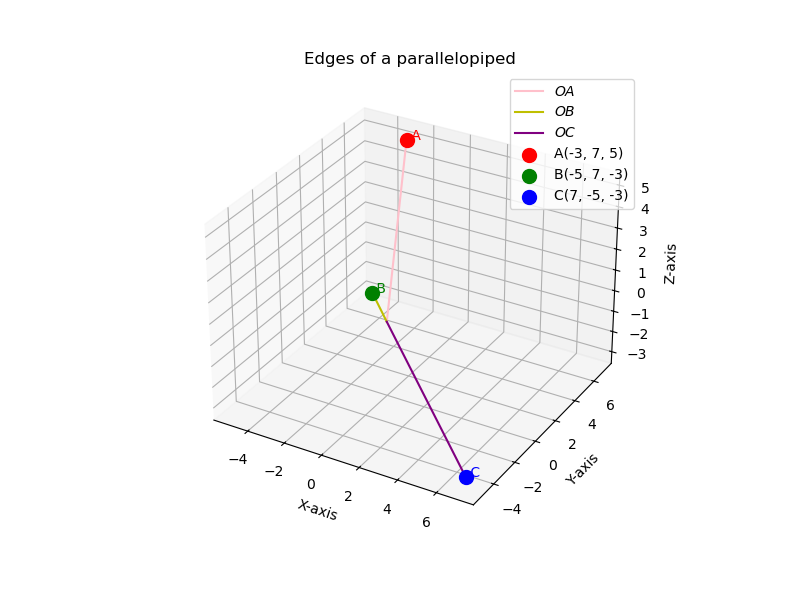
\includegraphics[scale=0.5]{plot}
	\caption*{}
	\label{fig}
\end{figure}
\end{document}
